\documentclass{scrartcl}
\usepackage{mm_ws15}
\usepackage{graphicx}

\newcommand{\sheetTitle}{Blatt 13, Abgabe 2.2.2016}
\begin{document}
\maketitle


%%%%%%%%%%%%%%%%%%%%%%%%%%%%%%%%%%%%%%%%%%%%%%%%%%%%%%%%%%%%%%%%%%%%%%%%%%%%%%%%
\section{Volumen einer Halbkugel \points{10}}
\label{sec:volumenintegral_i}

Wir betrachten eine Halbkugel mit Radius $a$ 
\[
  H = \{ (x,y,z) \in \RR^3 \, | \, x^2 + y^2 + z^2 \le a^2,\, z \ge 0 \}
\]
\begin{subex}
  \item\points{2} Zur Parametrisierung von $H$ in kartesischen Koordinaten überlegen Sie sich die folgenden Grenzen:
  \begin{enumerate}[label=\roman*)]
    \item $x$ läuft zwischen den Grenzen $x_1 \le x \le x_2$,
    \item $y$ läuft für gegebenes $x$ zwischen $y_1(x) \le y \le y_2(x)$
    \item $z$ läuft für gegebenes $x, y$ zwischen $z_1(x,y) \le z \le z_2(x,y)$.
  \end{enumerate}

  \item\points{3} Nutzen Sie die Ergebnisse aus a) für die Berechnung des Halbkugelvolumens in kartesischen Koordinaten
  \[
    V(H) = \int_H \dd V 
    = \int_{x_1}^{x_2} \dd x \int_{y_1(x)}^{y_2(x)} \dd y \int_{z_1(x,y)}^{z_2(x,y)} \dd z.
  \]

  \item\points{2} Überlegen Sie sich nun die Grenzen für die Parametrisierung $(r,\theta,\phi)$ in Kugelkoordinaten (siehe Vorlesung (5.30)).

  \item\points{3} Berechnen Sie das Volumen $V(H)$ mit Hilfe von Kugelkoordinaten.
\end{subex}

\begin{center}
    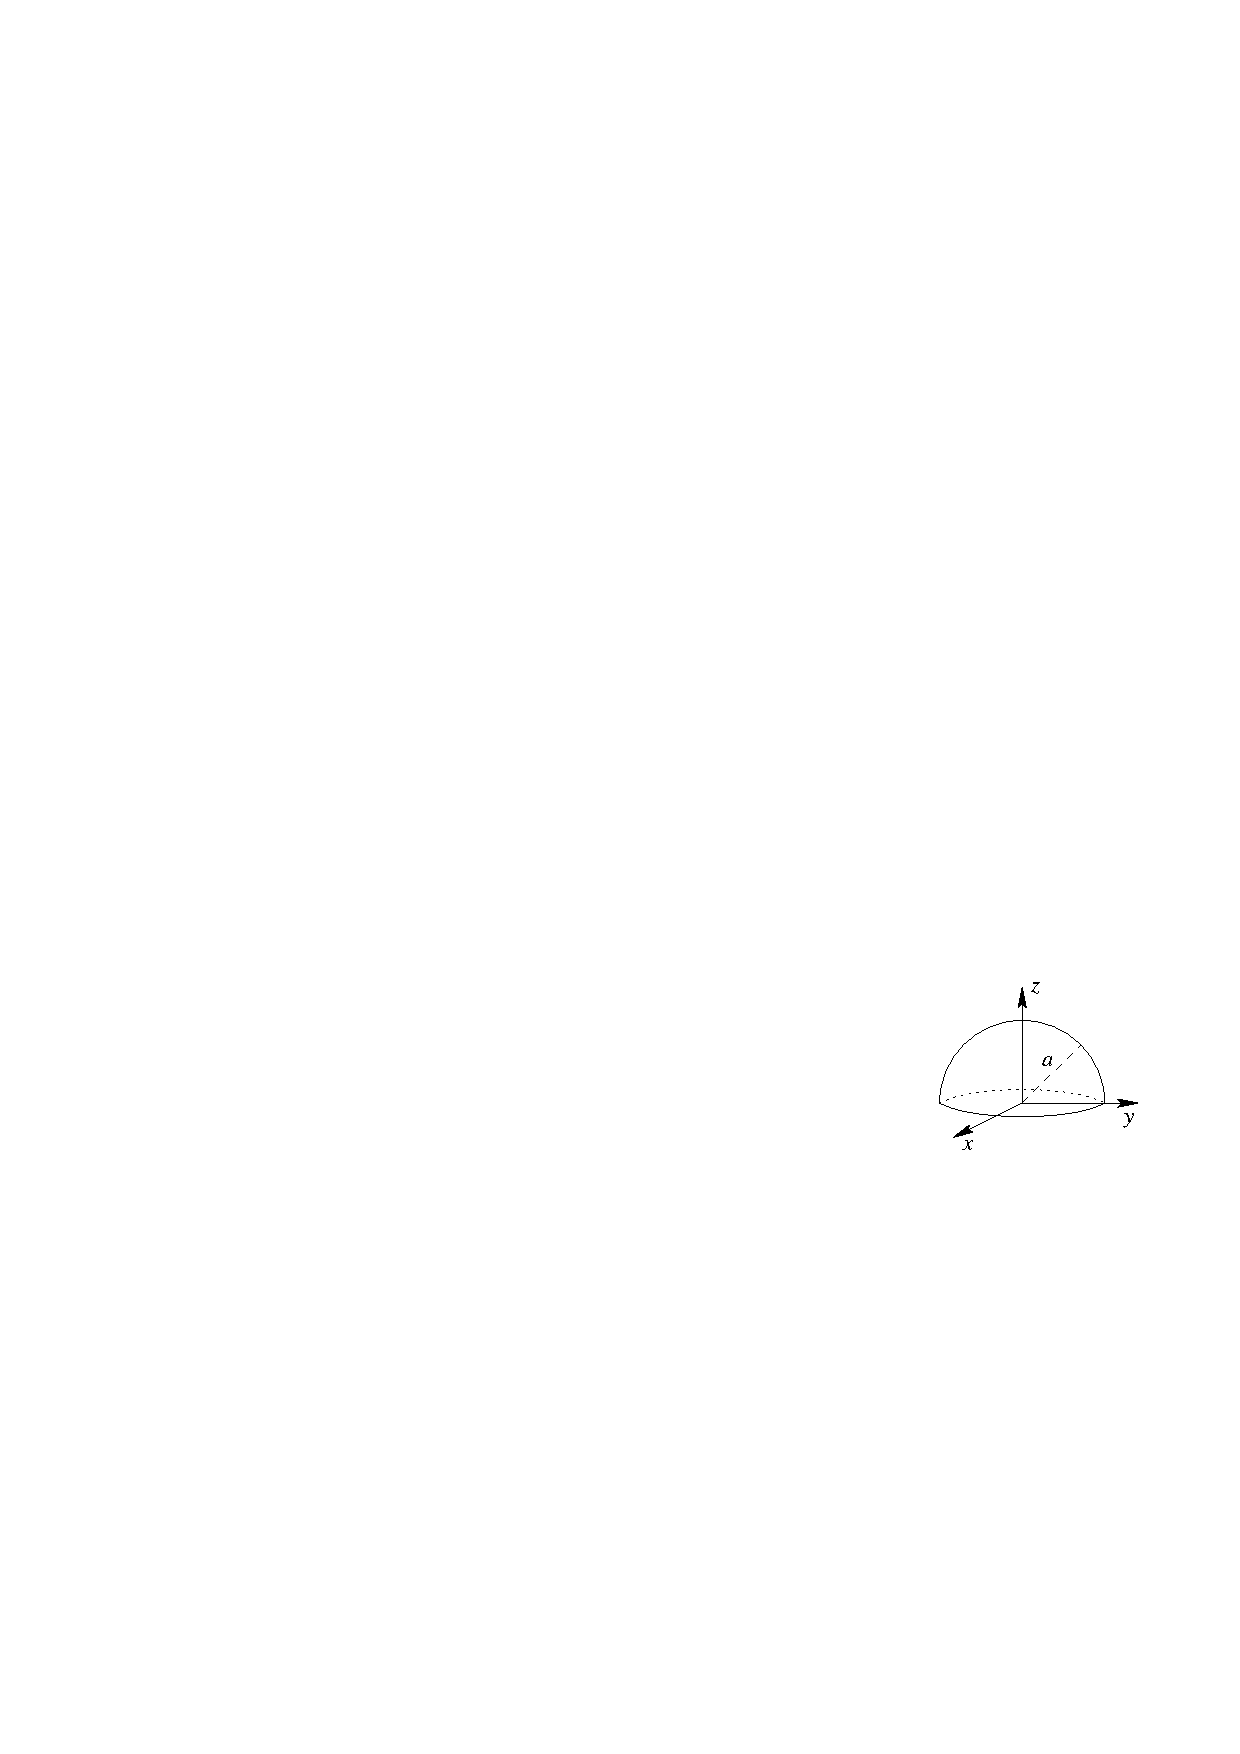
\includegraphics{img/semicircle.pdf}
    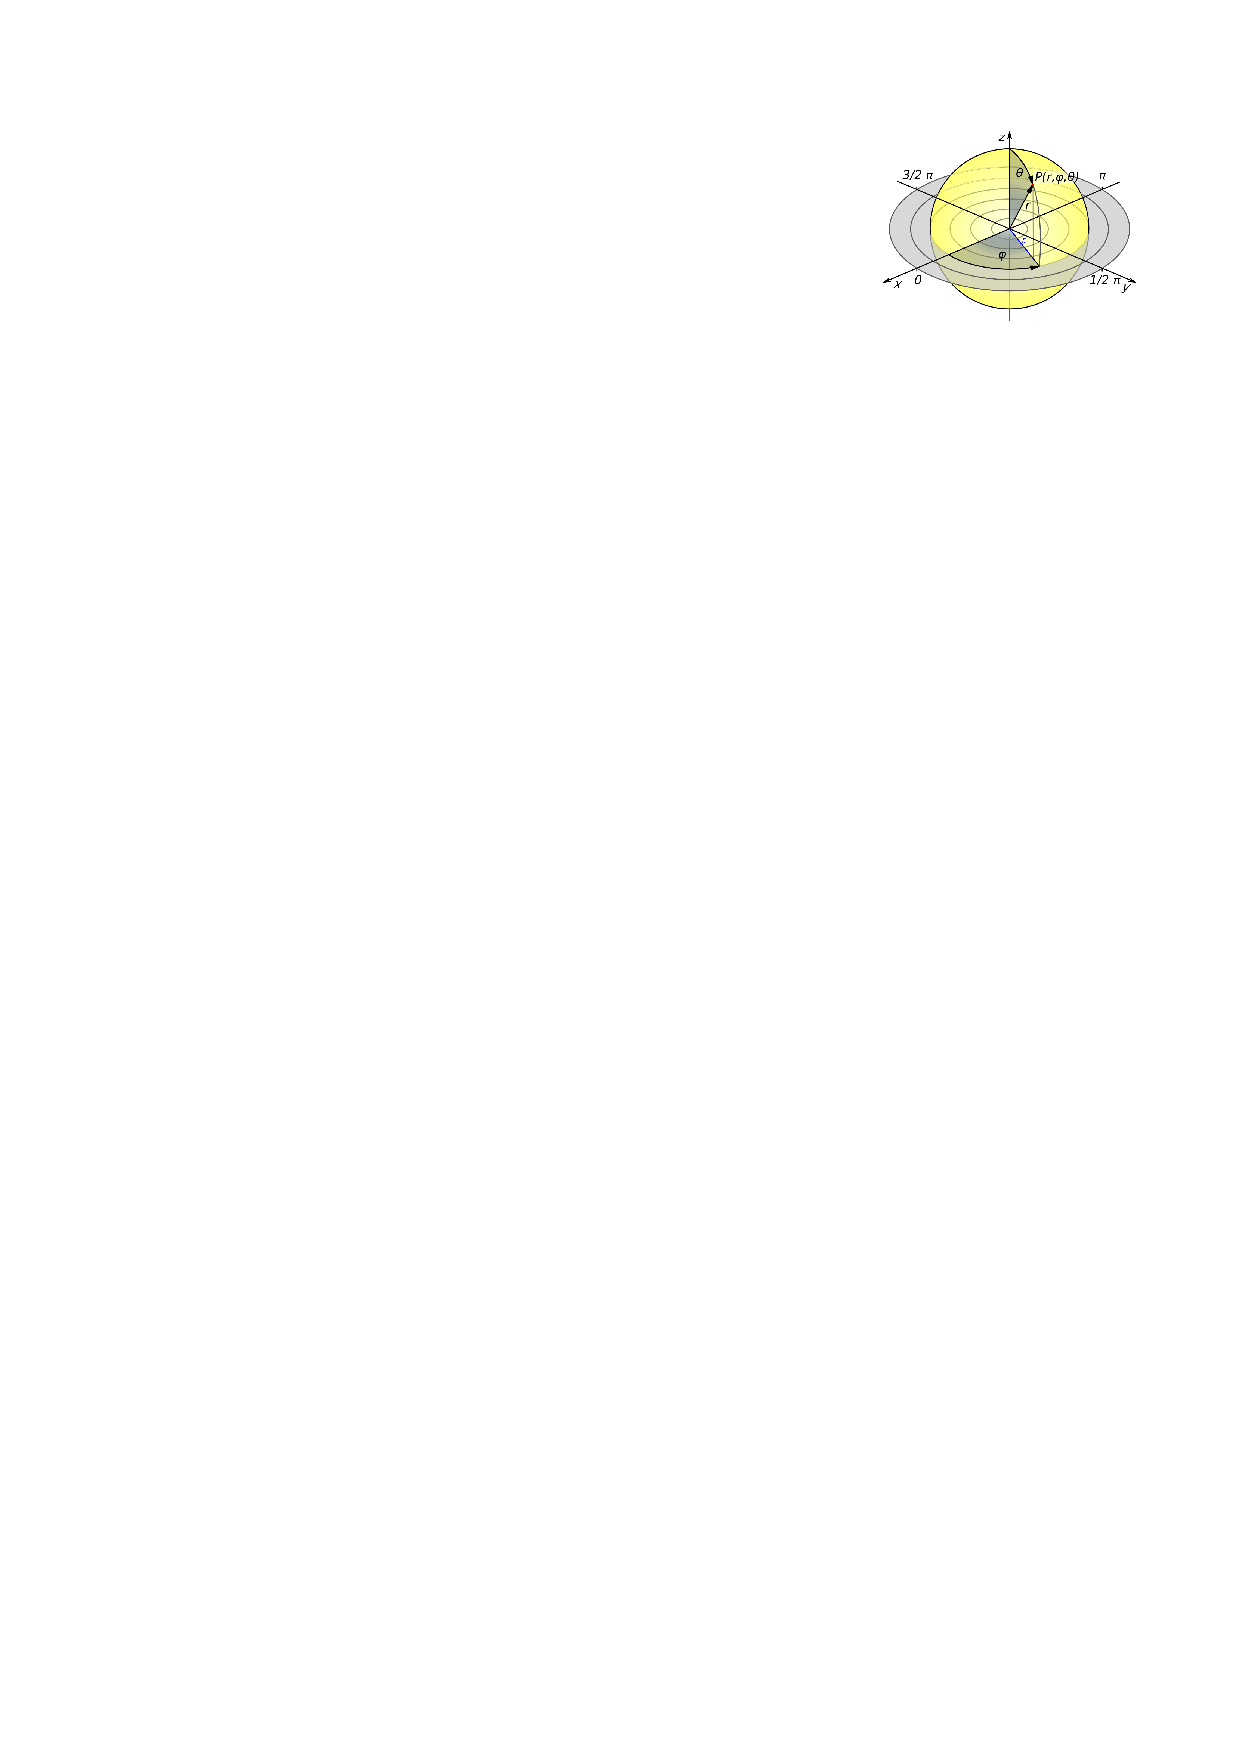
\includegraphics{img/sphere_coord.pdf}
\end{center}


%%%%%%%%%%%%%%%%%%%%%%%%%%%%%%%%%%%%%%%%%%%%%%%%%%%%%%%%%%%%%%%%%%%%%%%%%%%%%%%%
\section{Volumen und Oberfläche eines Kegels \points{10}}
\label{sec:volumenintegral_ii}

Wir betrachten einen Kreiskegel mit Grundflächenradius $b$ und Höhe $h$.
Zur Berechnung des Volumens des Körpers benutzen wir Zylinderkoordinaten $(\rho,\phi,z)$, die an die Symmetrie des Körpers angepasst sind
\[
  x = \rho \cos \phi, \quad y = \rho \sin \phi, \quad z = z.
\]
Hierbei ist $\rho$ der Abstand des Punktes zur $z$-Achse, $\phi$ der Azimutwinkel und $z$ der Abstand des Punktes zur $x-y$ Ebene.
\begin{subex}
  \item\points{2} Zeigen Sie, dass das Volumenelement in Zylinderkoordinaten gegeben ist durch
  \[
    \dd V = \rho \dd \rho \dd \phi \dd z.
  \]

  \item\points{2} Berechnen Sie das Volumen des Kreiskegels.

  \item\points{6} Berechnen Sie die Oberfläche des Kreiskegels mit Hilfe des Oberflächenintegrals.
\end{subex}
\begin{remark}{Hinweis}
  In Teilaufgabe c) beachten Sie, dass der Kreiskegel aus Mantel- und Grundfläche besteht.
  Finden Sie jeweils eine geeignete Parametrisierung und benutzen Sie Formel (5.22) der Vorlesung um die jeweilige Oberfläche zu berechnen.
\end{remark}

\begin{center}
  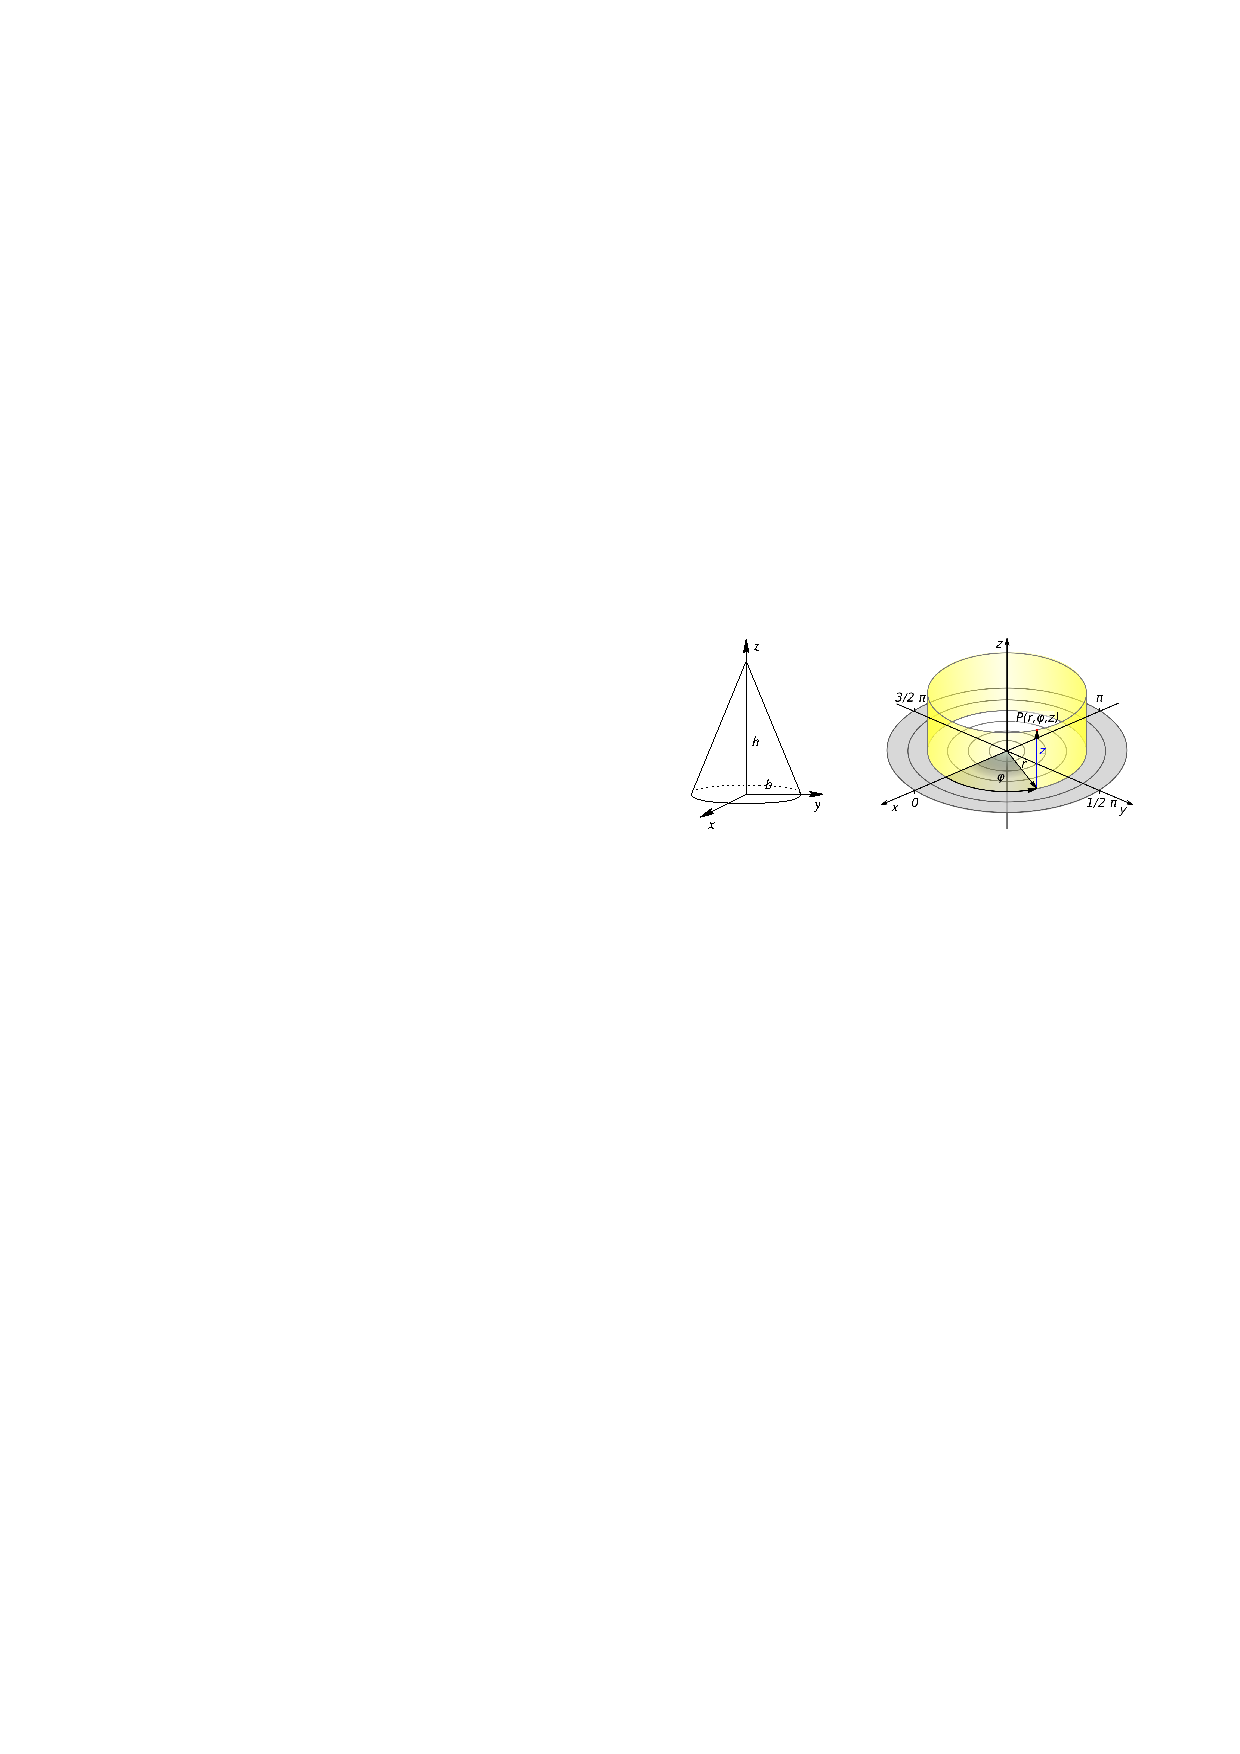
\includegraphics{img/cylinder.pdf}
\end{center}


%%%%%%%%%%%%%%%%%%%%%%%%%%%%%%%%%%%%%%%%%%%%%%%%%%%%%%%%%%%%%%%%%%%%%%%%%%%%%%%%
\section{Trägheitsmomente \points{10}}
\label{sec:tr_gheitsmomente}

Das Massenträgheitsmoment $J$ eines Körpers $K$ lässt sich bei bekannter Massendichte $\rho(\vec r)$ aus folgendem Volumenintegral berechnen
\[
  J = \int_K \dd V \, r_\perp^2 \, \rho(\vec r).
\] 
Hierbei bezeichnet $r_\perp$ den Abstand des Punktes \emph{zur Rotationsachse}.

\begin{subex}
  \item\points{5} Eine homogene Kugel $K$ mit Masse $m$ und Radius $r$ rotiert um die $z$-Achse. 
  Zeigen Sie, dass für das Trägheitsmoment gilt
  \[
    J_z = \frac{3 m}{4\pi r^3}\, \int_K \dd V \, (x^2 + y^2). 
  \]
  Berechnen Sie $J$.
  \item\points{5} Ein hohler Zylinder mit Innenradius $r_1$, Außenradius $r_2$ ($r_1 < r_2$), Höhe $h$ und Gesamtmasse $m$ rotiert um seine Symmetrieachse.
  Berechnen Sie das Massenträgheitsmoment.
\end{subex}

\begin{center}
  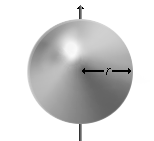
\includegraphics[width=.3\textwidth]{img/Traegheit_j_kugel1-2.png}
  \hspace{1cm}
  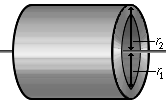
\includegraphics[width=.3\textwidth]{img/Traegheit_d_hohlzylinder2.png}
\end{center}

\let\thefootnote\relax\footnotetext{%
  Bildquellen:\\
  \noindent\url{http://de.wikipedia.org/wiki/Kugelkoordinaten}\\
  \url{http://de.wikipedia.org/wiki/Polarkoordinaten#Zylinderkoordinaten}\\
  \url{http://de.wikipedia.org/wiki/Trägheitsmoment}
}

\end{document}